%%%%%%%%%%%%%%%%%%%%%%%%%%%%%%%%%%%%%%%%%
% Journal Article
% LaTeX Template
% Version 1.1 (25/11/12)
%
% This template has been downloaded from:
% http://www.LaTeXTemplates.com
%
% Original author:
% Frits Wenneker (http://www.howtotex.com)
%
% License:
% CC BY-NC-SA 3.0 (http://creativecommons.org/licenses/by-nc-sa/3.0/)
%
%%%%%%%%%%%%%%%%%%%%%%%%%%%%%%%%%%%%%%%%%

%----------------------------------------------------------------------------------------
%   PACKAGES AND OTHER DOCUMENT CONFIGURATIONS
%----------------------------------------------------------------------------------------

\documentclass[twoside]{article}

\usepackage[english]{babel}
\usepackage{graphicx}

\usepackage{lipsum} % Package to generate dummy text throughout this template

\usepackage[sc]{mathpazo} % Use the Palatino font
\usepackage[T1]{fontenc} % Use 8-bit encoding that has 256 glyphs
\linespread{1.05} % Line spacing - Palatino needs more space between lines
\usepackage{microtype} % Slightly tweak font spacing for aesthetics



\addtolength{\oddsidemargin}{-.875in}
\addtolength{\evensidemargin}{-.875in}
\addtolength{\textwidth}{1.75in}
\addtolength{\topmargin}{-.875in}
\addtolength{\textheight}{1.75in}

\usepackage[hmarginratio=1:1,top=26mm,columnsep=20pt]{geometry} % Document margins
\usepackage{multicol} % Used for the two-column layout of the document
\usepackage{hyperref} % For hyperlinks in the PDF

\usepackage[hang, small,labelfont=bf,up,textfont=it,up]{caption} % Custom captions under/above floats in tables or figures
\usepackage{booktabs} % Horizontal rules in tables
\usepackage{float} % Required for tables and figures in the multi-column environment - they need to be placed in specific locations with the [H] (e.g. \begin{table}[H])

\usepackage{lettrine} % The lettrine is the first enlarged letter at the beginning of the text
\usepackage{paralist} % Used for the compactitem environment which makes bullet points with less space between them

\usepackage{abstract} % Allows abstract customization
\renewcommand{\abstractnamefont}{\normalfont\bfseries} % Set the "Abstract" text to bold
\renewcommand{\abstracttextfont}{\normalfont\small\itshape} % Set the abstract itself to small italic text

\usepackage{titlesec} % Allows customization of titles
%\renewcommand\thesection{\Roman{section}}
\titleformat{\section}[block]{\large\scshape\centering}{\thesection.}{1em}{} % Change the look of the section titles

%\usepackage{fancyhdr} % Headers and footers
%\pagestyle{fancy} % All pages have headers and footers
%\fancyhead{} % Blank out the default header
%\fancyfoot{} % Blank out the default footer
%\fancyhead[C]{Running title $\bullet$ November 2012 $\bullet$ Vol. XXI, No. 1} % Custom header text
%\fancyfoot[RO,LE]{\thepage} % Custom footer text

%----------------------------------------------------------------------------------------
%   TITLE SECTION
%----------------------------------------------------------------------------------------

\title{\vspace{-15mm}\fontsize{24pt}{10pt}\selectfont\textbf{L.U.M.P.}} % Article title

\author{
    \large
    \textsc{Mason Silber \quad Vivek Bhagwat}\\[2mm] % Your name
    \normalsize Columbia University \\ % Your institution
    \normalsize \{mds2161,vsb2110\}@columbia.edu % Your email address
    \vspace{-5mm}
}
\date{}

%----------------------------------------------------------------------------------------

\begin{document}

\maketitle % Insert title

%\thispagestyle{fancy} % All pages have headers and footers

%----------------------------------------------------------------------------------------
%   ARTICLE CONTENTS
%----------------------------------------------------------------------------------------

\begin{multicols}{2} % Two-column layout throughout the main article text

%----------------------------------------------------------------------------------------
%   ABSTRACT
%----------------------------------------------------------------------------------------

\begin{abstract}

\noindent \lipsum[1] % Dummy abstract text

\end{abstract}
Abstract

\section{Introduction}
Locks may be one of the most pervasive technologies in the world. Traditional, physical locks are used for houses, cars, windows, fences, and luggage – every object in the world humans deem worth protecting. However, it was not always just objects themselves that were worth protecting --- it was information as well.\\

There are a few examples of this type of information security --- the first is physically protecting information by putting it in a safe with a dial, such that turning the dial the correct amount in the correct direction a few times in sequence allows access to the contents of a box. This design allows for physical valuables to be stored in such a way that makes it only accessible to those who have knowledge of the correct sequence of physical manipulations of a lock. \\

The second type, which is more relevant in our increasingly electronic world, is the obfuscation of information through means such as ciphers, which encodes information in such a way that can only be decoded if the reader knows the algorithm, or cipher, which allows them to change the form into a human-readable format. This method is much older than the computing technology ubiquitous today, however. Classical ciphers, for example, simply substitute letters with other letters (e.g. G is always replaced with L). However, the problems with this sort of cipher is that it is easy to figure out an algorithm when it is simple and efficient to calculate, either by human or computer. This is the motivation behind symmetric and asymmetric encryption, which drives a great deal of authentication today. \\
\\
Symmetric-key encryption algorithms are ones in which the same key is used for both encryption and decryption. This means that this key must be present for both the reader and writer, and agreed upon in advance. However, if the key is sufficiently complex, this allows for a simple and quick algorithm which still is inefficient and difficult to decipher for any third parties. Today, algorithms such as the Advanced Encryption Standard (AES) employ this form of encryption. The main problem, however, is that both parties must know the key in advance. This makes AES perfectly acceptable for situations in which data are simply being encrypted for reading later, not transferred securely. \\
\\
When transferring data over a medium which another party could potentially read, asymmetric-key encryption is preferred. Asymmetric-Key encryption is system in which users are able to share a “public key” insecurely with the intended recipient of some encrypted data. Additionally, a “private key” is generated for each of the two parties involved in the transfer such that the keys can be combined to make the data only readable to those who have the correct private and public key. This algorithm prevents anyone who has access to all data being transferred to be able to decrypt the data, because that user’s private key will not be able to combine with the public key which has been distributed to allow access to the encrypted data. This type of encryption is pervasive across many types of systems, including HTTPS, which uses SSL with HTTP.  It is this implementation of asymmetric-key encryption that is relevant to this paper.\\

In the physical world, however, we cannot simply use numbers to protect our valuables. This is the reasons safes still exist and are so widely used, and is one of the motivations of this project --- to combine the convenience of software security and the protection of lockboxes. Traditionally, identity can be verified in some subset of “what you know,” “what you have,” and “who you are.” Software security implementations as described above generally rely on the “what you know” aspect (e.g. passwords, public and private keys, etc.) of identity verification while traditional locks rely on “what you have” (i.e. physical keys for a physical lock). As a result, companies  such as Google, Dropbox, and Twitter have recently begun implementing two-step verification for logging into their services. These verification processes usually rely on knowledge of a password as well as ownership of a smartphone, which provides a temporal code which can be entered into the service as a second step in the authentication process. \\

The ability to rely on both these forms of identity verification allows for a more robust security system, and the ubiquity of technologies such as smartphones makes these implementations have far-reaching effects.\\

\section{Overview of iOS and Arduino and Raspberry Pi}

\subsection{iOS}

\begin{figure}[H]
\centering
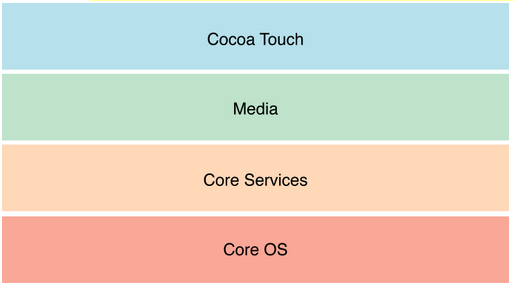
\includegraphics[width=0.5\textwidth]{ios_arch.png}
\caption{iOS Architecture}
\end{figure}

iOS is a closed-source, mobile operating system developed by Apple, Inc., and is one of the most popular mobile operating systems in the world. iOS runs on iPhone, iPod, iPad, and AppleTV; as of June 2012, over 400 million devices worldwide were running iOS. \\

\\
iOS architecture has an architecture made up of four layers. The top layer is Cocoa Touch, which provides developers with standardized user interface objects such as buttons, sliders, table views, and other commonly used components. Cocoa Touch also provides abstractions from lower-level functionality in a number of frameworks. Native frameworks exist for audio processing, animation and graphics development, networking, and persistent storage, among others. As its name suggests, Cocoa Touch also provides access to all touch events that occur on the device. \\
The next layer is the Media layer. The media layer provides lower level access to audio, video, graphics, and animation functionality and processing. Frameworks such as Core Text, Core Image, Core MIDI, and GLKit exist in this layer. \\
Below the Media layer is the Core Services layer. Core Services provides access to iCloud technologies, a system by which user information and data can be automatically synced in the cloud using key-value storage. The Core Services layer also facilitates Automatic Reference Counting, relieving developers of most of the responsibility of memory management. Core Services provides developers with the ability to pass blocks of code as function parameters. This functionality allowed for the implementation of a C library called Grand Central Dispatch (GCD), which makes multithreaded app development much simpler. Frameworks like the Accounts Framework (access to Twitter and Facebook), the Ad Support Framework, and the Foundation Framework. \\
The last layer of the iOS architecture is the Core OS layer. Core OS provides access to external hardware attachments and internal hardware components, such as the bluetooth receiver and the accelerometer. The Core OS layer also provides developers with security libraries and basic access to system calls. \\

\begin{figure}[H]
\centering
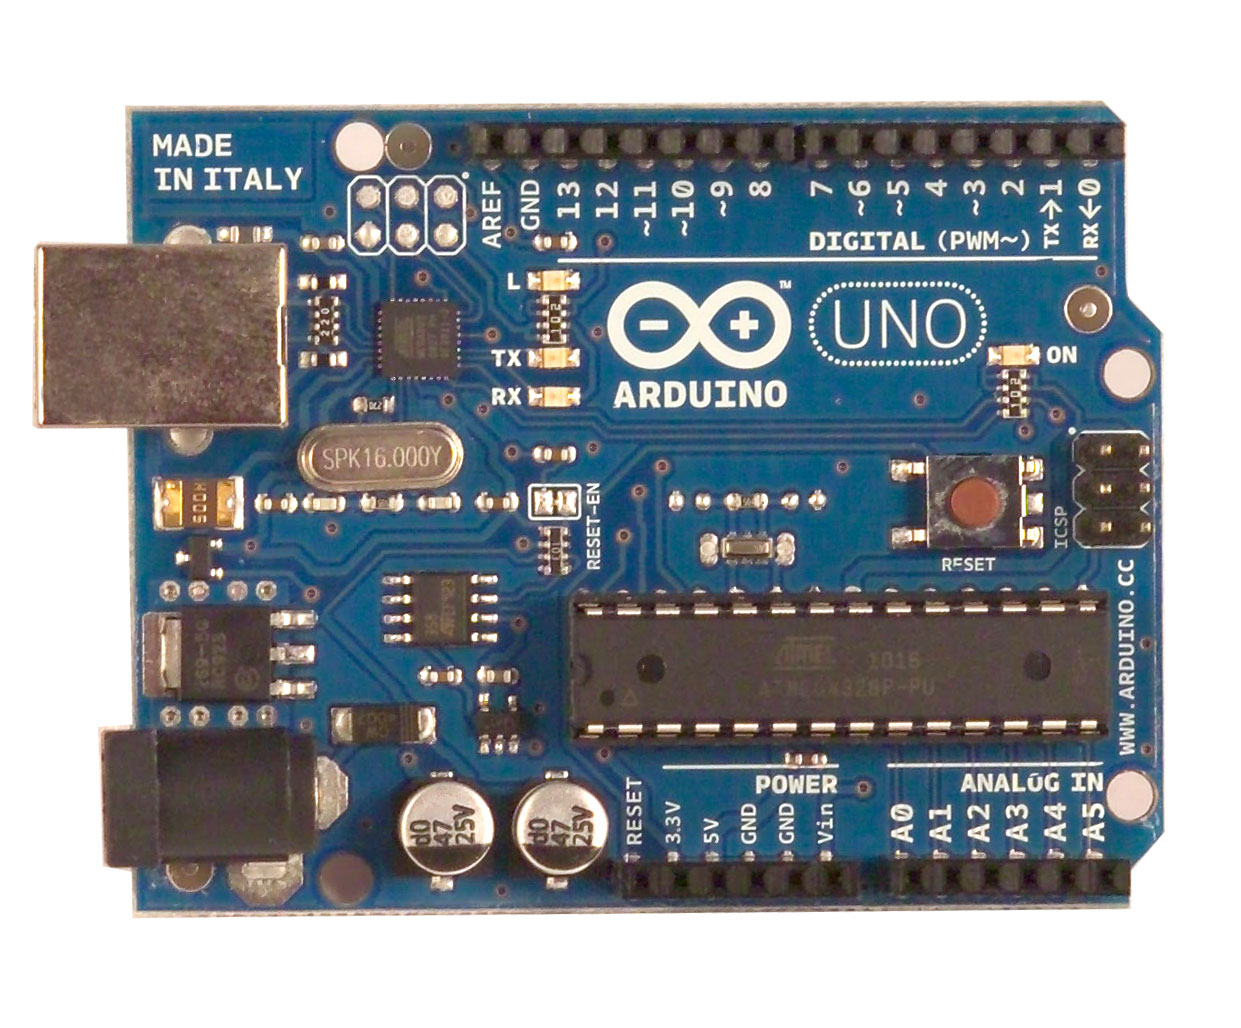
\includegraphics[width=0.5\textwidth]{arduino.jpg}
\caption{Arduino Uno}
\end{figure}
\\
\subsection{Arduino Uno}
Arduino is an open-source microcontroller designed with the intention of making hardware development more accessible. Because we used an Arduino Uno in our experimental setup, we will limit our discussion to that particular model. \\

The Arduino Uno is a board designed around the ATmega328 microcontroller. It has 32 kb of flash memory, 2 kb of SRAM, and 1 kb of EEPROM. There are 14 digital I/O pins and 6 analog in pins, which can be controlled or read by the microcontroller. Six of the digital I/O pins are also able to emit Pulse Width Modulated (PWM) signals, which are used to control motors and other components. The Arduino is powered with a 5V power supply, either from a USB port or an AC to DC converter. \\

However, what truly differentiates Arduino from other microcontrollers is the presence of a bootloader. Whereas normal microcontrollers often need an external programmer to load a program onto the chip before it’s placed on the circuit board, Arduino’s bootloader allows C programs to be uploaded directly from the developer’s machine to the microcontroller’s flash memory. This allows the code to be executed immediately, and streamlines development. \\

Aside from loading programs directly into the microcontroller’s flash memory, serial directives can be sent over USB to the Arduino using a protocol called Firmata. We use this approach in our experimental design with our secure server, which handles user requests. \\
\\

Figure 3: Raspberry Pi Model B

\subsection{Raspberry Pi}
The Raspberry Pi is an open source, low cost, single board computer developed by the Raspberry Pi Foundation. Two models currently exist, Model A and Model B. We used a Model B Raspberry Pi in our experimental setup, so we won’t discuss Model A. \\
At a price of just \$35, the Model B Raspberry Pi is one of the cheapest computers on the market. It ships with an 800MHz ARM processor, 512 MB of RAM, audio and video out, an Ethernet jack, two USB ports, an HDMI port, 26 GPIO pins, and an SD card slot. It runs many distributions of Linux, including Arch Linux ARM, Debian, Fedora, and others. For this project we chose to use Raspbian OS, a distribution of Debian designed specifically for the Raspberry Pi. \\
\\
\subsection{Firmata}
    Firmata is an open-source protocol used to communicate between a computer and a microcontroller. The computer sends serial data via USB (or some other connector) to the microcontroller, and receives serial data in response. Firmata allows microcontrollers to be significantly augmented by much more powerful computers, and can be very useful in situations in which some heavy computation is being performed. \\
        Libraries exist to communicate with Arduino through Firmata in many languages, including Perl, Python, Ruby, Java, and Javascript. All of these libraries are open source as well, and abstract away many of the low level difficulties associated with Firmata. \\
\\

        \subsection{BreakfastSerial}
            BreakfastSerial is an open-source Python library that facilitates serial communication between a computer and an Arduino through Firmata. BreakfastSerial includes abstractions for Arduino boards, LEDs, push button switches, RGB LEDs, Sensors, and Servo Motors. During our work on this project, we actually contributed to BreakfastSerial by implementing the abstraction for the Servo component, which we needed for our experimental setup. \\
            Normally, Arduino programming must be done in C, a barrier which many people find tough to breach. Libraries like BreakfastSerial alleviate people of this responsibility by creating a way to develop for Arduino in higher level languages. In our experiment, we created a Python HTTPS server to handle locking and unlocking requests, so BreakfastSerial is an ideal library for our purposes. \\
\\
            \section{Experimental Setup}

            \subsection{Client Side}
            Our client application is an iOS app, titled Lockbox. Lockbox is a very simple app that lists a user’s locks and whether each lock is currently locked or unlocked. The app also facilitates in-app additions of new locks, using a single, simple form. \\
            Lockbox launches by prompting the user to enter a four digit PIN, in order to access their locks. If this is the first time the app is being launched, the user will be required to input a four digit PIN, which is stored securely in the iPhone’s keychain. \\
            Upon a successful entry of the PIN, the app launches into the home screen, which is simply a list of locks\\
\\
            \section{Results}

            \section{Related Work}
            Wireless networked security has become a popular entrepreneurial venture in the last few years. Many companies have announced locks you can control with a remote, from your phone, or simply by walking up to the door. \\
            One of the most notable companies to market a similar product is Lockitron. Lockitron provides a wireless electronic lock for normal doors. Controlled via a smartphone app or a text message, Lockitron locks allow users to lock and unlock their doors from anywhere, get notifications whenever their door is locked or unlocked, distribute expiring keys (bed and breakfasts may use this, for example). \\
            However, Lockitron’s solution costs \$179 to pre order, and only works for doors. Our solution addresses a more general problem. Our implementation could be used on doors as well, but also on safes, lock boxes, cars, and anything else with a locking and unlocking mechanism. The simplicity of the servo implementation allows for easy, adaptable extensions for locks on nearly anything.\\
\\
            \section{Conclusions}

            \section{Future Work}

            \section{Acknowledgments}


%------------------------------------------------


%----------------------------------------------------------------------------------------
%   REFERENCE LIST
%----------------------------------------------------------------------------------------

\begin{thebibliography}{99} % Bibliography - this is intentionally simple in this template

\bibitem[Figueredo and Wolf, 2009]{Figueredo:2009dg}
Figueredo, A.~J. and Wolf, P. S.~A. (2009).
\newblock Assortative pairing and life history strategy - a cross-cultural
study.
\newblock {\em Human Nature}, 20:317--330.

\end{thebibliography}

%----------------------------------------------------------------------------------------

\end{multicols}

\end{document}

